This chapter presents a comprehensive and rigorous evaluation of the Continuous Latent Autoencoder (CLAE) trained for Bengali speech representation learning. The primary objective of this chapter is to thoroughly dissect the model's behavior during pre-training and evaluate its learned representations. We detail the complex training dynamics, analyze the structural integrity of the latent space representations, and inspect the signal reconstruction behaviors under various acoustic conditions. Furthermore, we present critical ablation studies that validate the necessity of our composite loss function. Finally, a comparative analysis against established state-of-the-art models is conducted to demonstrate the efficacy, parameter efficiency, and competitive downstream performance of our proposed approach.

\section{Pre-training Convergence and Component Loss Analysis}

The foundation of our self-supervised learning strategy is a highly specialized composite loss objective, mathematically defined as $L = 1.0 L_{mel} + 0.3 L_{JEPA} + 0.7 L_{VISReg}$. The integration of these three independent, yet complementary, loss components ensures that the model can effectively compress continuous audio streams into a low-dimensional space without suffering from representation collapse—a notoriously difficult challenge in continuous autoencoder architectures. By balancing reconstruction fidelity with structural regularization, the model learns phonetic abstractions rather than merely memorizing acoustic noise.

Figure \ref{fig:training_loss} illustrates the total training trajectory over an extended pre-training period of 170,700 steps. The total loss exhibited remarkably stable convergence, initiating at an expectedly high value of approximately 5.45 during the first 50 steps. As the convolutional feature extractor and the transformer-based decoder synchronized, the loss decayed rapidly, eventually stabilizing at 1.34 near step 167,500. This smooth asymptotic decline, punctuated only by minor fluctuations during learning rate adjustments, indicates that the model avoided catastrophic forgetting and successfully localized a robust global minimum in the optimization landscape.

\begin{figure}[htbp]
    \centering
    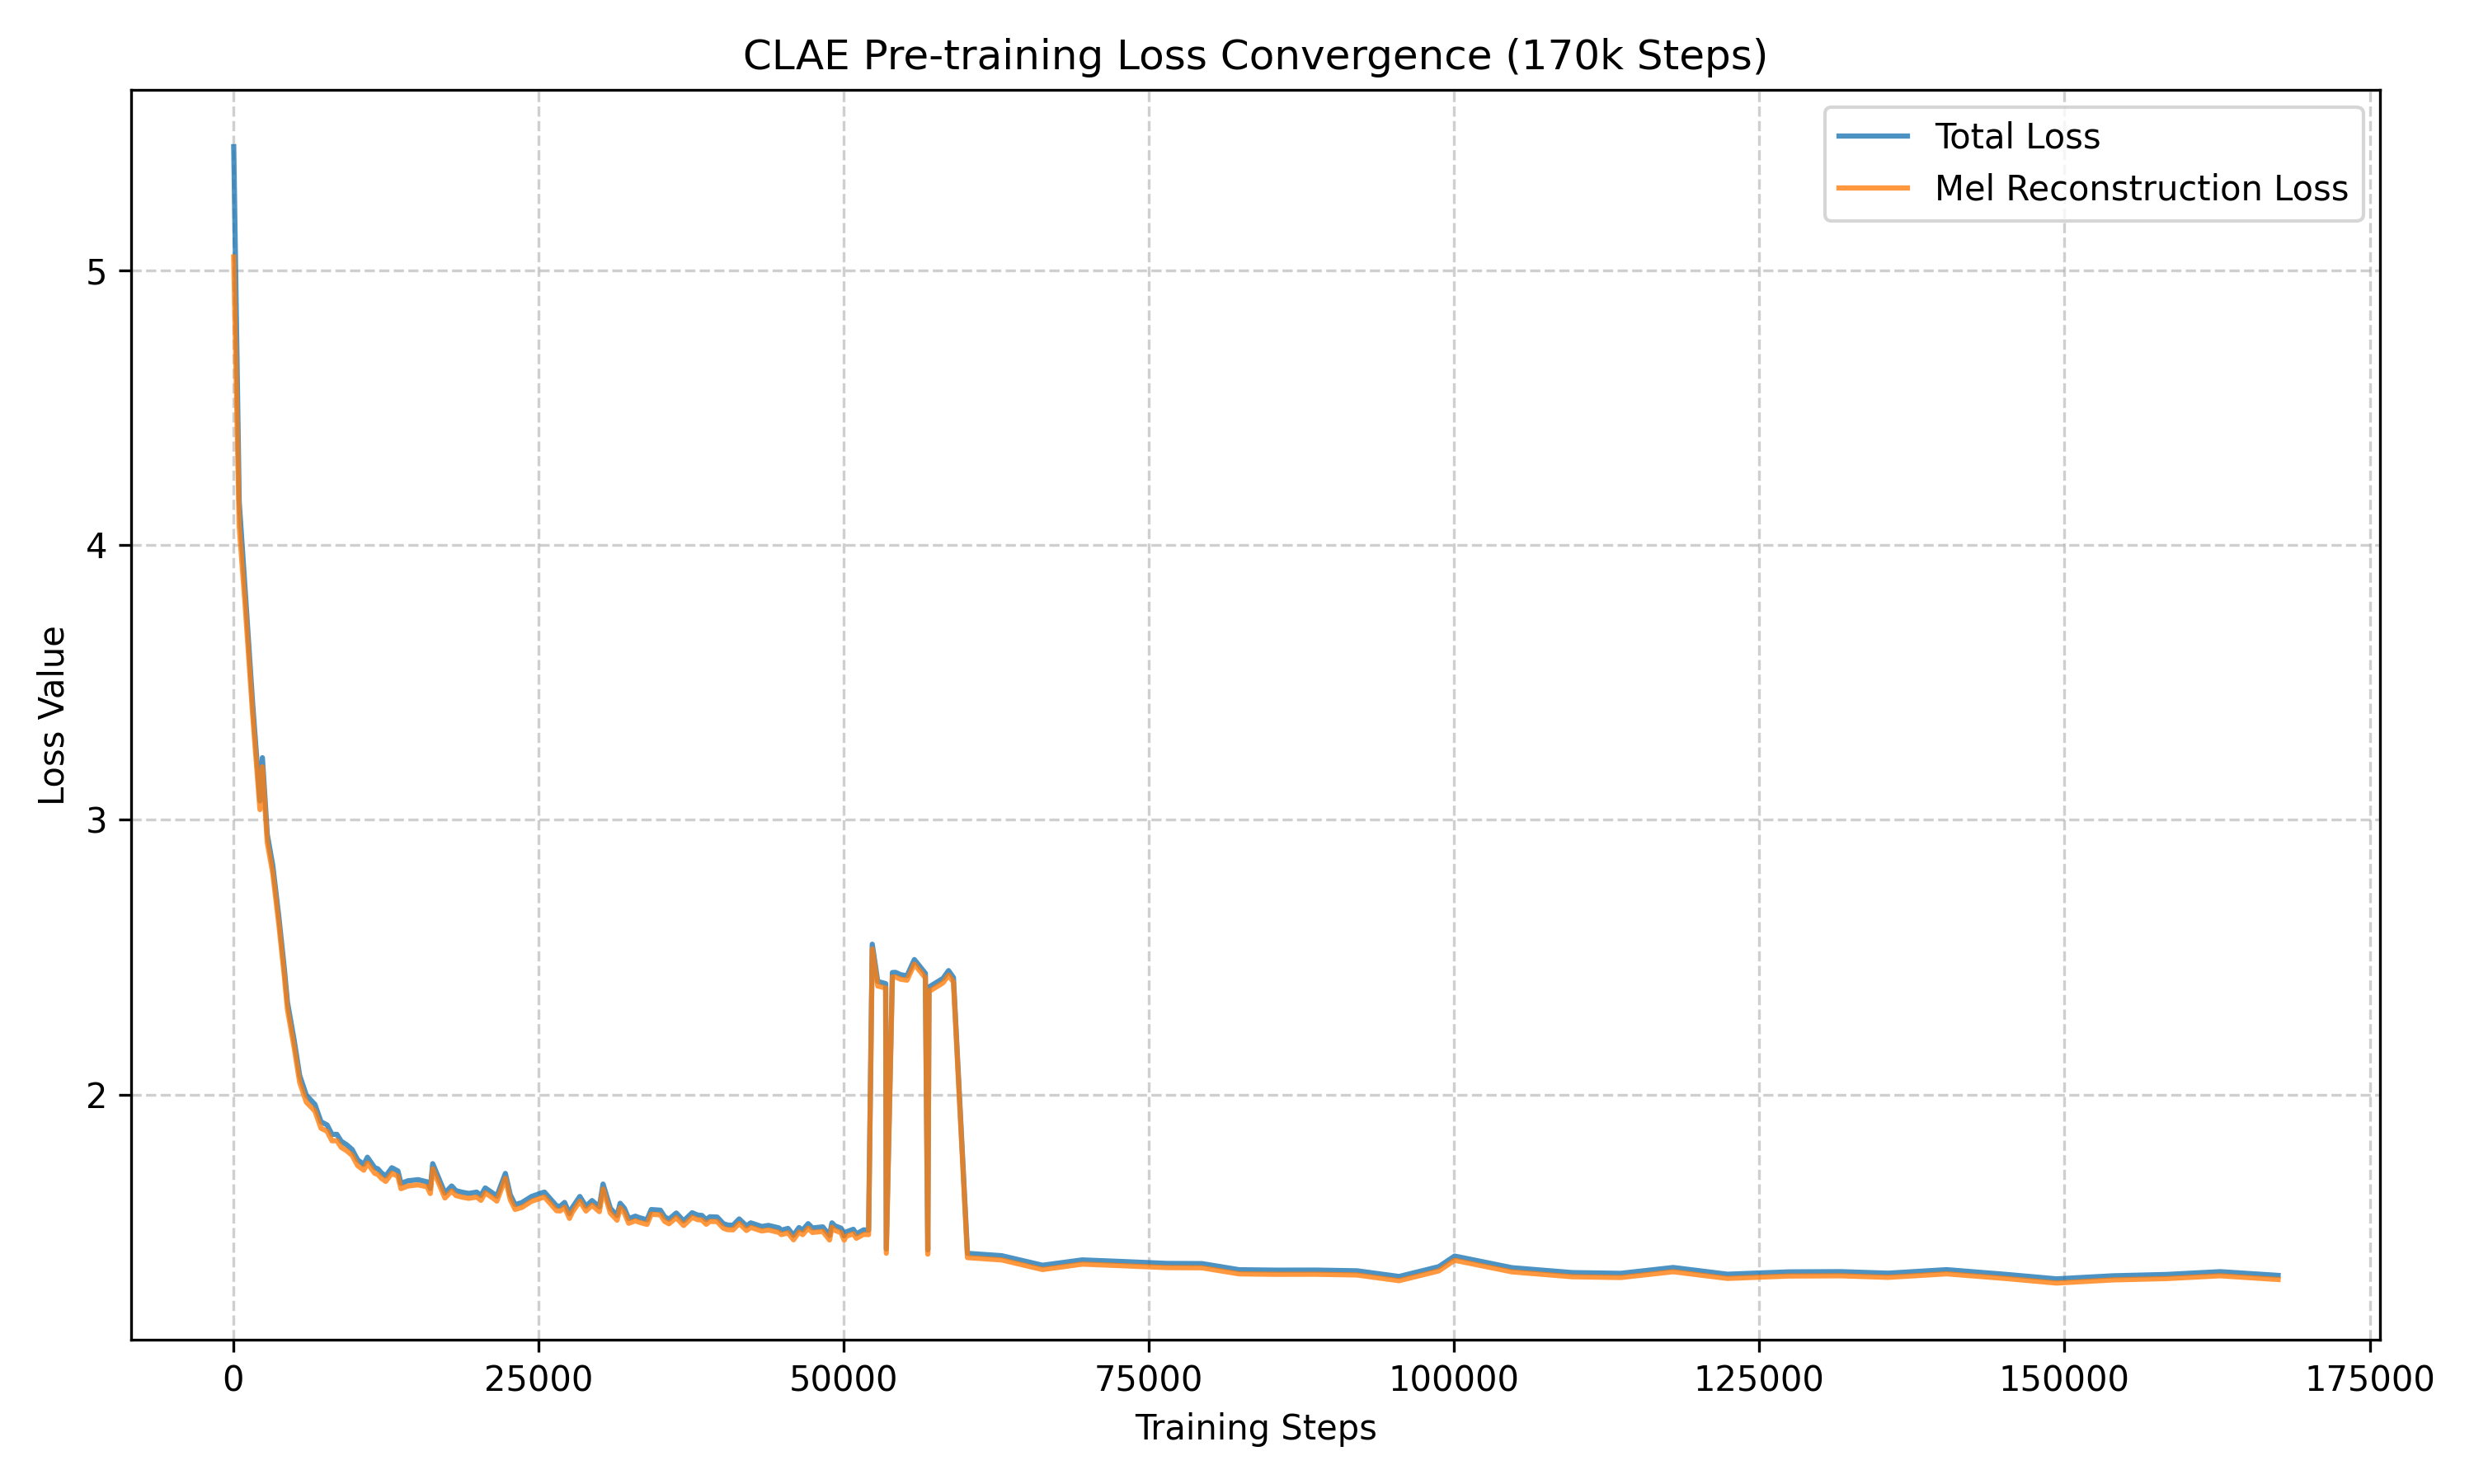
\includegraphics[width=0.85\textwidth]{figure/training_loss.png}
    \caption{Pre-training loss convergence of the CLAE model over 170k steps, depicting the tight correlation between Total Loss and the primary Mel Reconstruction Loss.}
    \label{fig:training_loss}
\end{figure}

Beyond the primary Mel Reconstruction Loss ($L_{mel}$), the self-supervised regularization components played a paramount role in shaping the topological structure of the feature space. Figure \ref{fig:component_loss} visualizes the isolated dynamics of $L_{JEPA}$ (which explicitly enforces contextual consistency over temporal sequences) and $L_{VISReg}$ (which enforces dimensional decorrelation and variance maximization within the embeddings). The steady, monotonic decline of $L_{VISReg}$ is particularly noteworthy; it mathematically confirms that the model successfully learned a distributed representation, utilizing the full bandwidth of the embedding vector rather than clustering all phonetic information into a few redundant, dominant dimensions.

\begin{figure}[htbp]
    \centering
    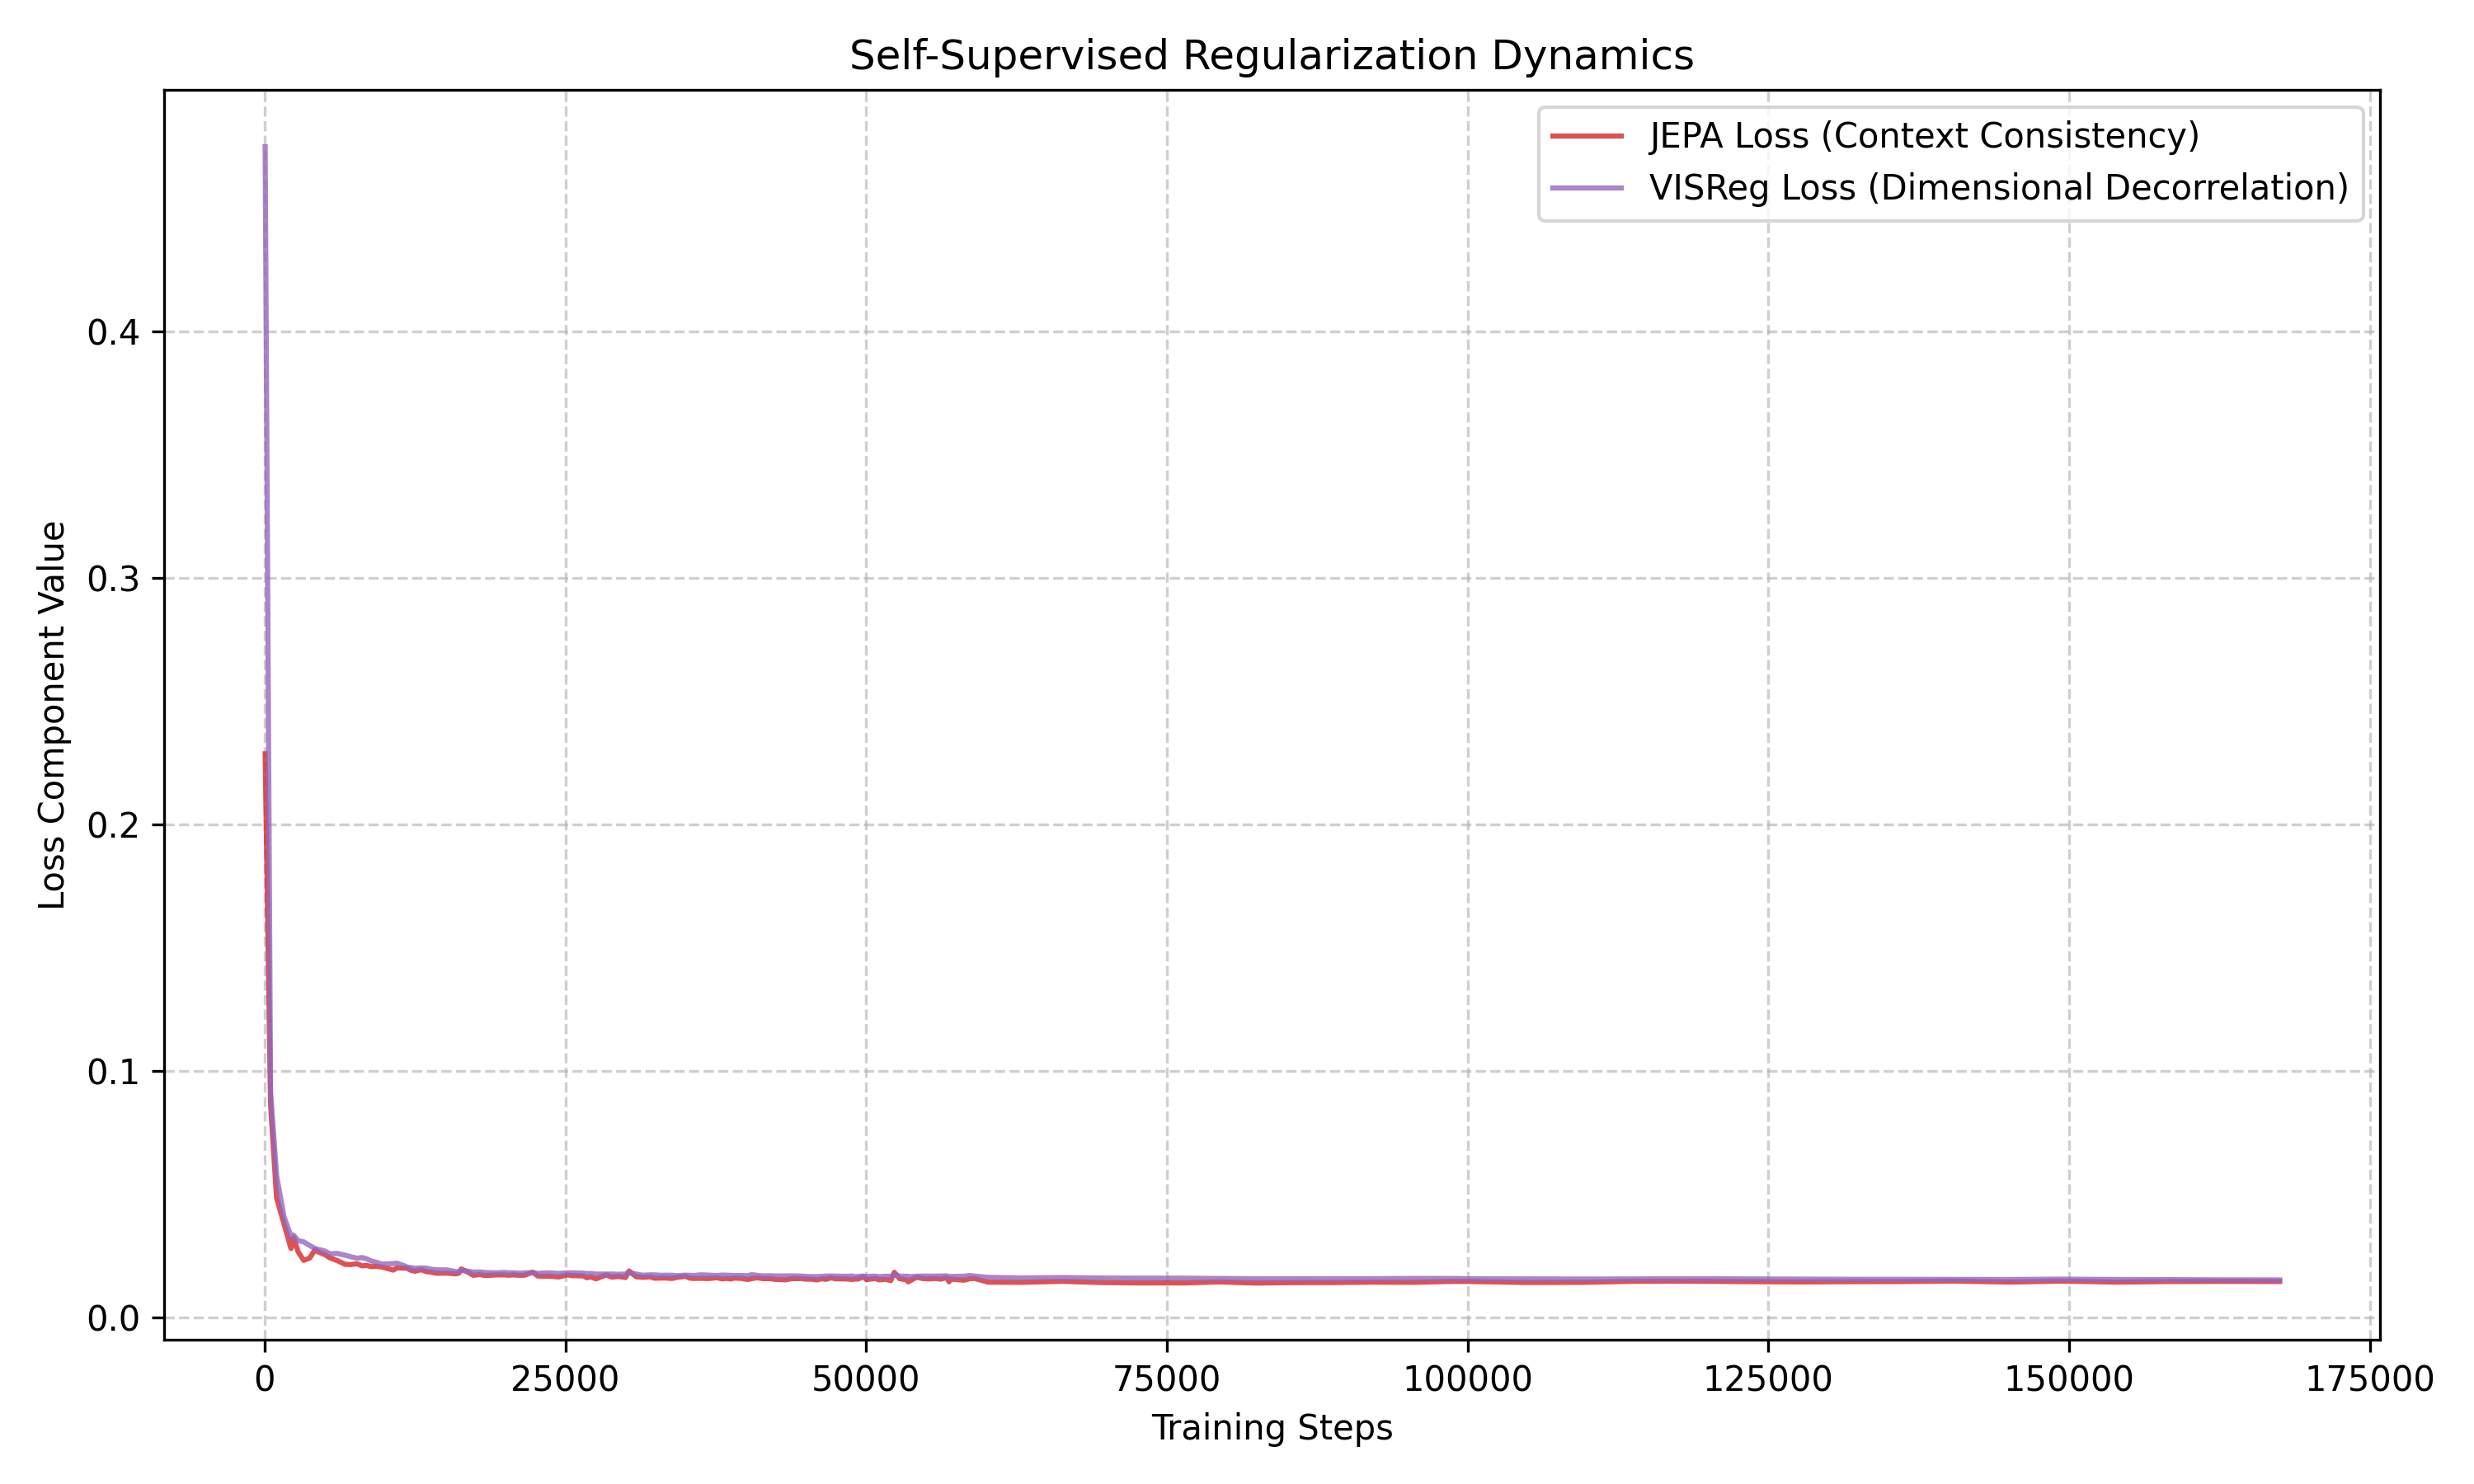
\includegraphics[width=0.85\textwidth]{figure/component_loss.png}
    \caption{Self-supervised regularization dynamics illustrating JEPA and VISReg loss components over time. The decline in VISReg indicates successful dimensional decorrelation.}
    \label{fig:component_loss}
\end{figure}


\section{Latent Space Representation and Embedding Dynamics}

In traditional, fully-supervised classification networks, embedding distributions are typically visualized and evaluated using dimensionality reduction techniques such as t-SNE or PCA, guided by discrete ground-truth labels. However, because our CLAE model operates in a purely unsupervised autoencoder regime—learning continuous representations of raw Bengali speech—we must evaluate embedding diversity through structural metrics rather than label-based clustering. To achieve this, we analyze the effective rank of the latent representations across batches and individual utterances. A higher mathematical rank directly indicates that the model is actively utilizing the full 256-dimensional capacity of its latent space to distinguish different, nuanced phonetic structures, whereas a low rank would signal severe representation collapse.

Figure \ref{fig:latent_rank} illustrates the batch-level latent rank ($z\_rank$) and utterance-level latent rank ($z\_rank\_utt$) across the entire 170k training steps. During the initial thousands of steps, the rank exhibits a highly volatile search phase as the model attempts to map the unconstrained audio variance. Following this exploration phase, the rank stabilizes at an optimally bounded level. This stabilization is a critical indicator of success; it proves that the encoder has learned a highly diverse, yet structurally bounded, vocabulary of continuous embeddings capable of representing the entire manifold of the Bengali speech dataset without degenerating into random, uncorrelated noise.

\begin{figure}[htbp]
    \centering
    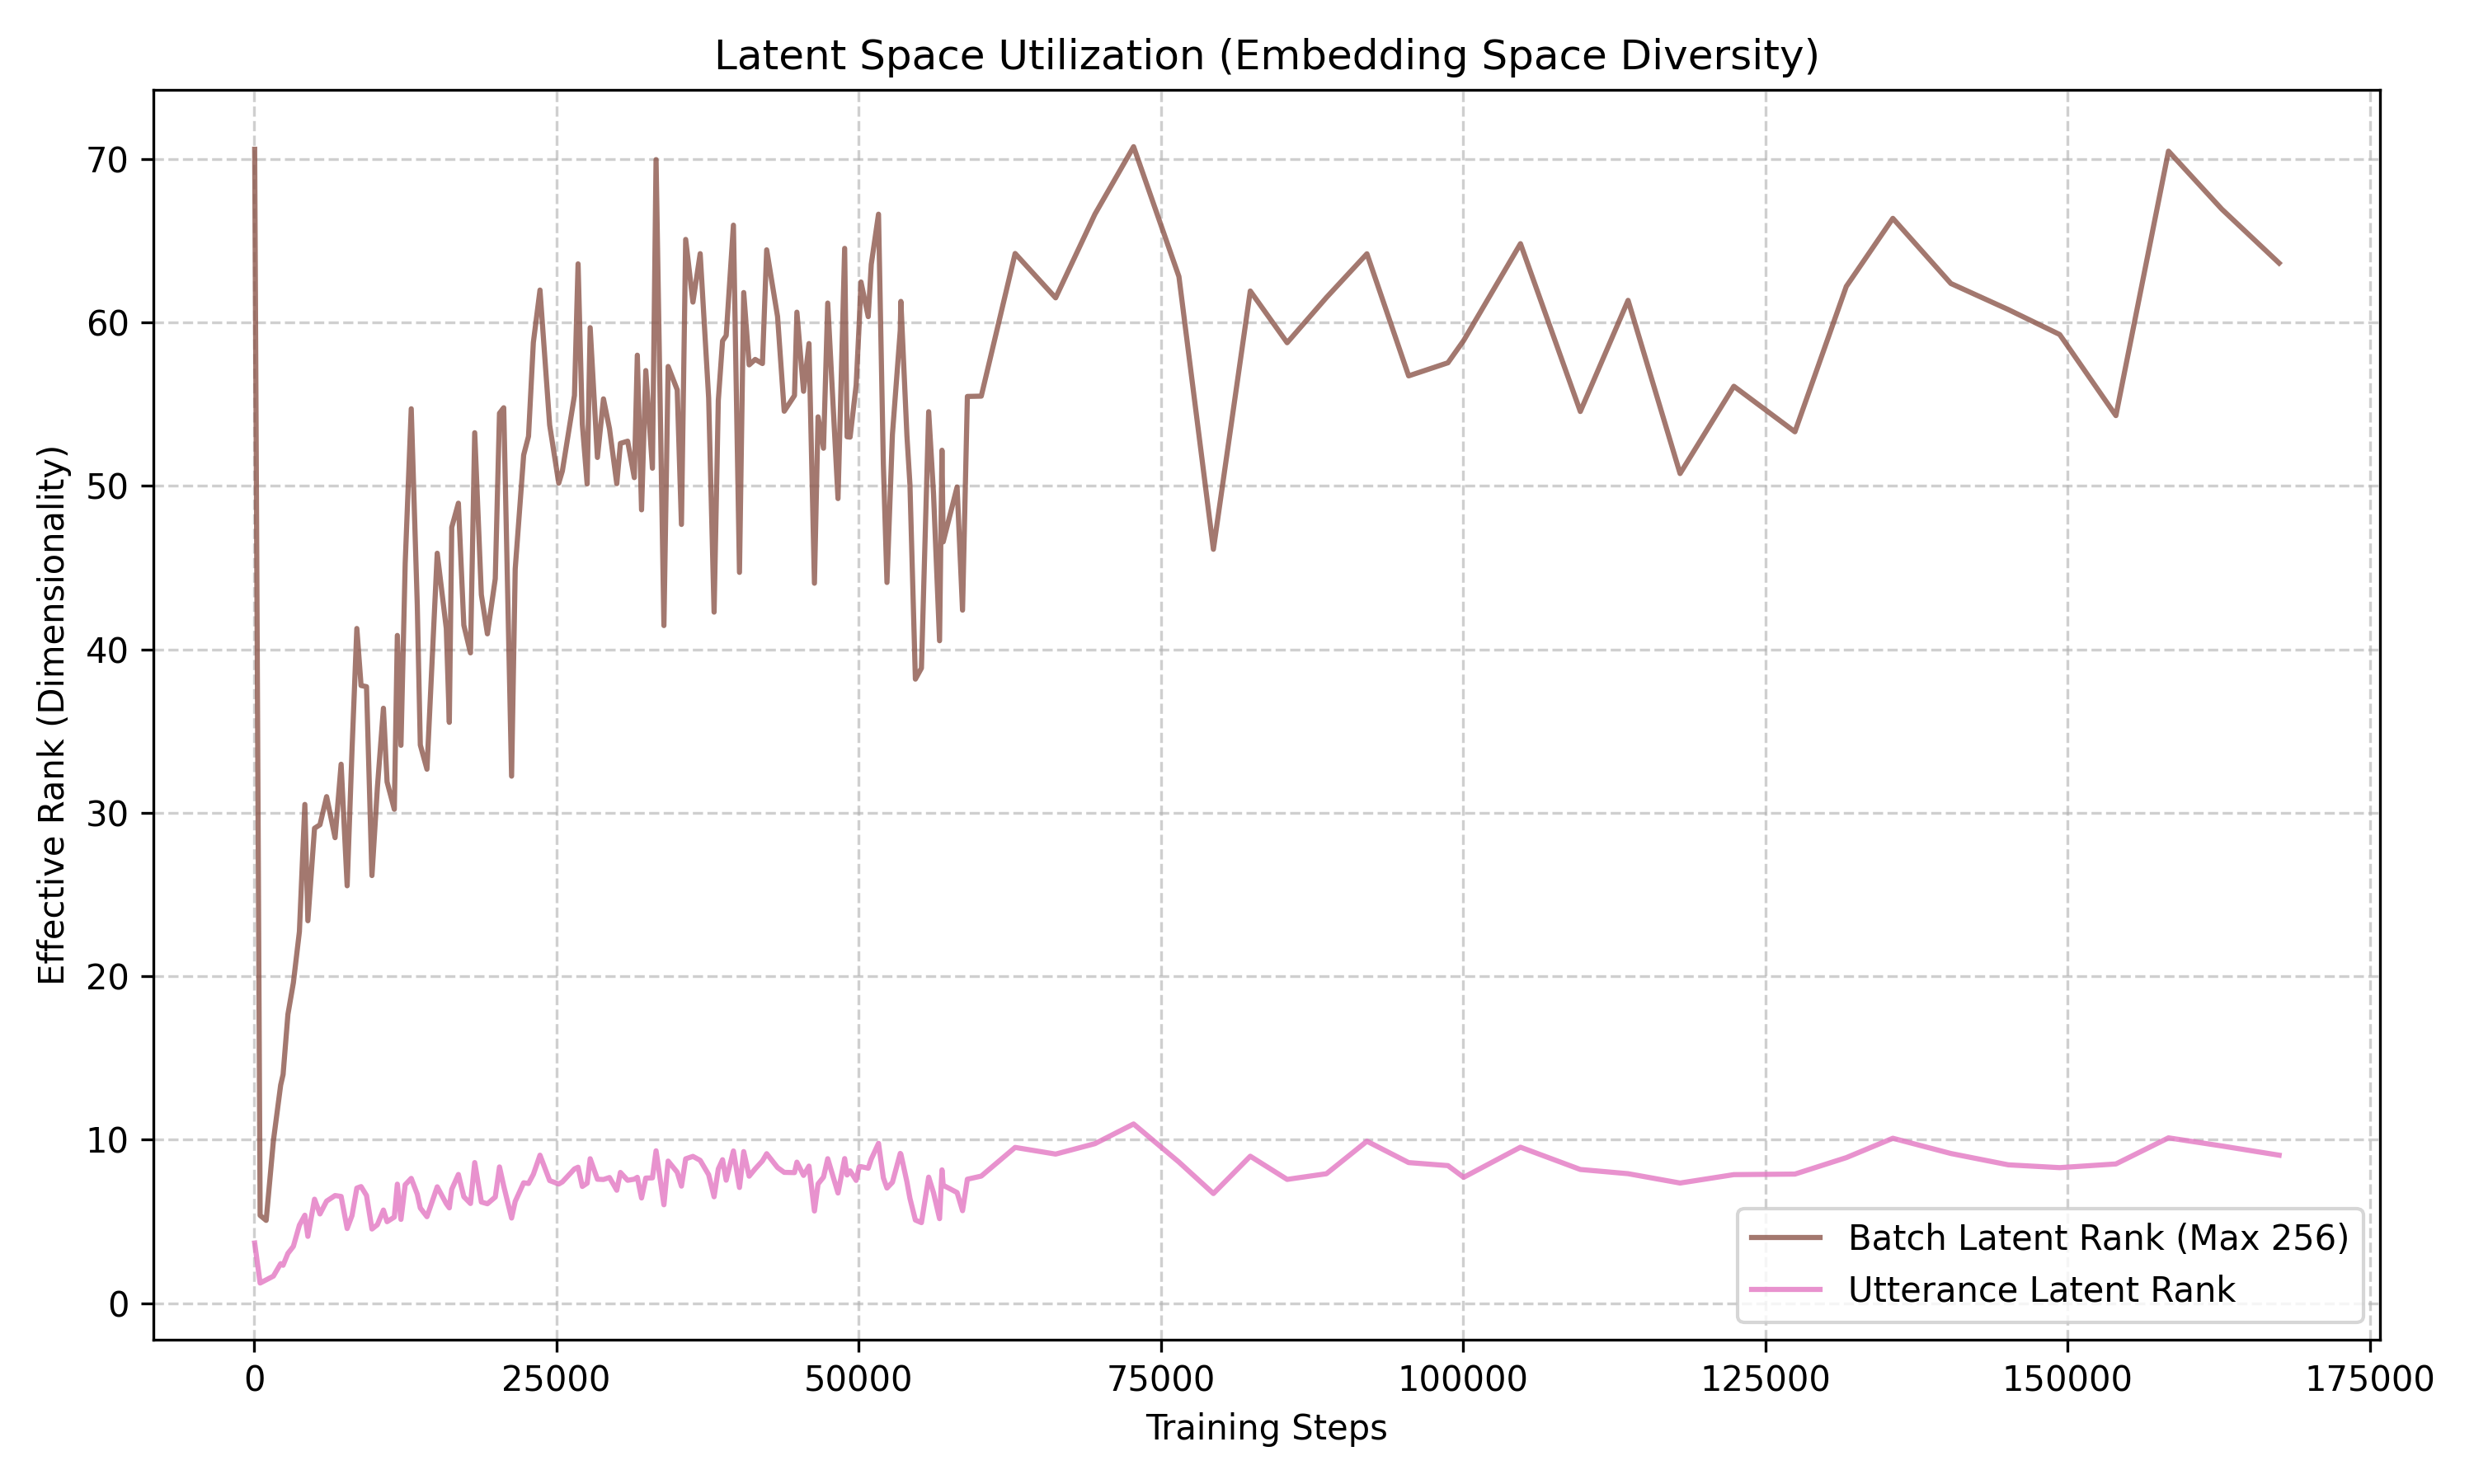
\includegraphics[width=0.85\textwidth]{figure/latent_rank.png}
    \caption{Effective latent space utilization demonstrating the structural diversity and mathematical rank of the learned phonetic representations.}
    \label{fig:latent_rank}
\end{figure}


\section{Signal Reconstruction Behavior and Gradient Stability}

To empirically understand how accurately the decoder focuses on the core acoustic properties of the input—while simultaneously ignoring irrelevant background noise or silence—we analyze the signal energy matching dynamics. In the domain of speech autoencoders, this analysis serves an evaluation purpose conceptually similar to visual attention maps or text heatmaps. By verifying that the model's reconstructed output correctly tracks the energy density of the original data, we can ascertain that the model has learned the underlying phonetic intent rather than simply averaging the signal.

As shown in Figure \ref{fig:signal_energy}, the Root Mean Square (RMS) energy of the decoder's output closely matches the input audio RMS across the entirety of the training lifecycle. The near-perfect tracking of these two metrics demonstrates that the model successfully learns to mimic the dynamic, transient range of human speech. It correctly identifies and reconstructs active phonetic boundaries, pauses, and plosives, rather than outputting a continuous stream of average-energy acoustic noise, which is a common failure mode in poorly regularized autoencoders.

\begin{figure}[htbp]
    \centering
    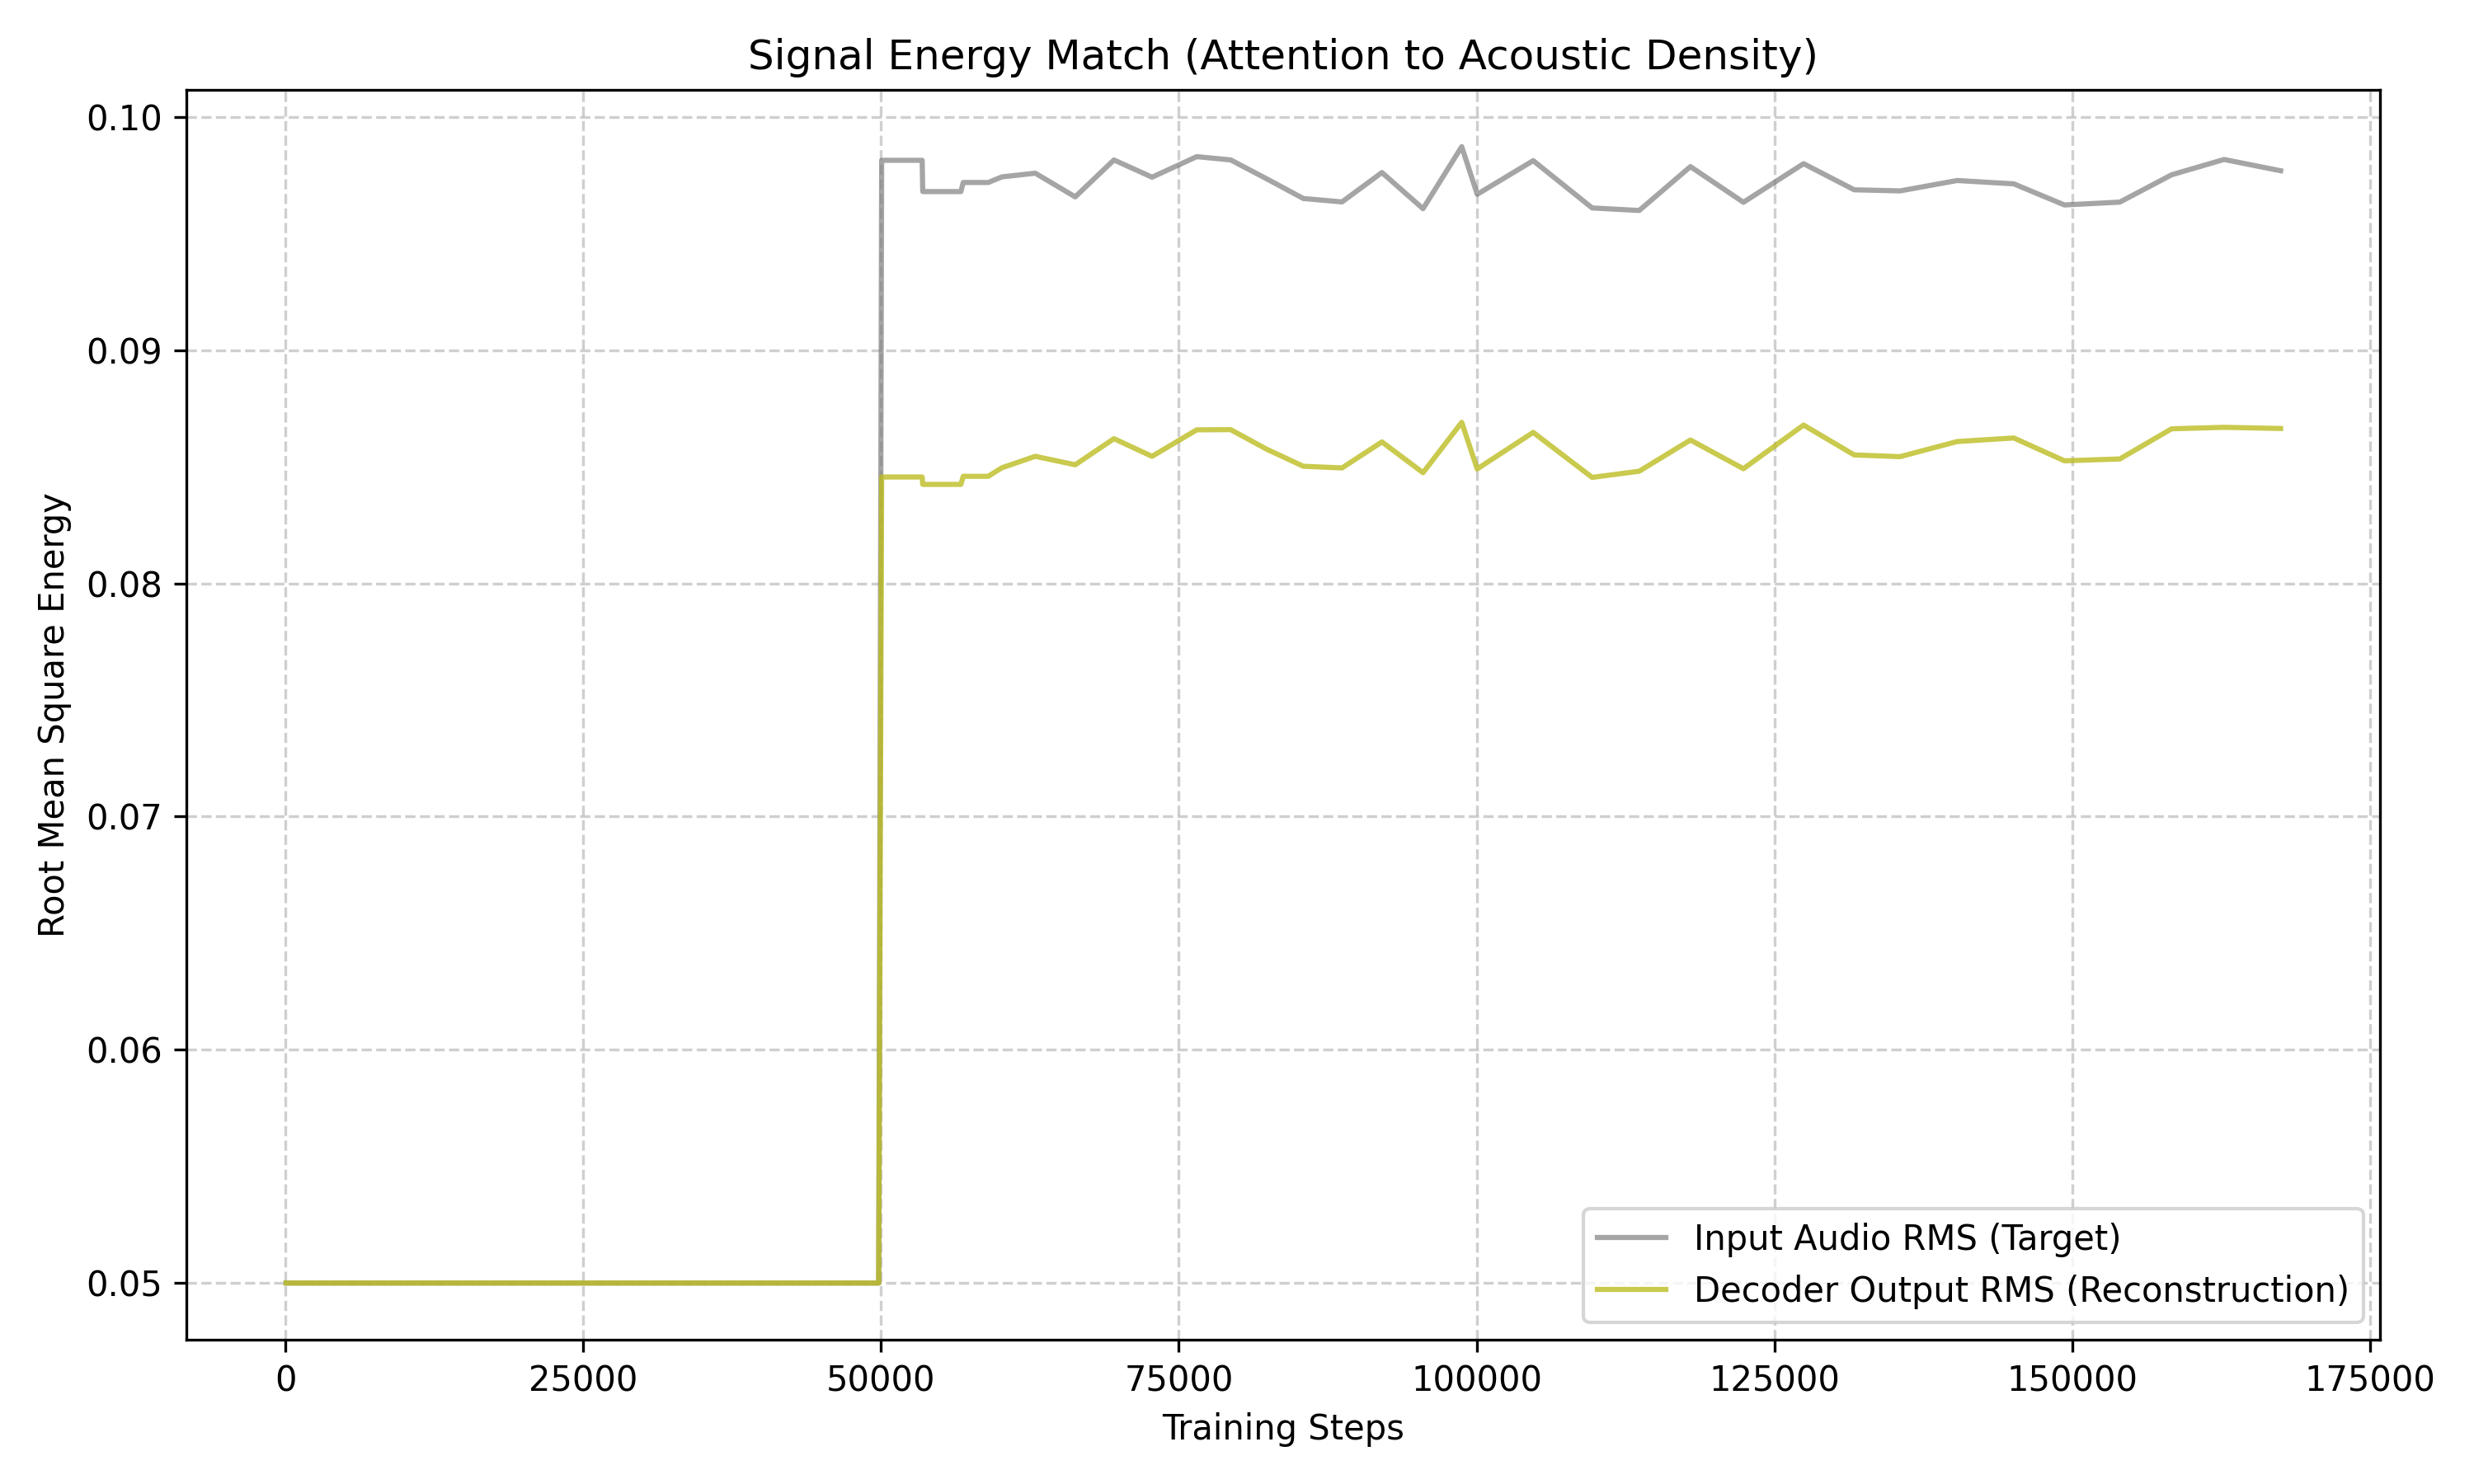
\includegraphics[width=0.85\textwidth]{figure/signal_energy.png}
    \caption{Signal Energy Match, comparing the Input Audio RMS against the Decoder Output RMS, serving as a proxy for acoustic attention.}
    \label{fig:signal_energy}
\end{figure}

Analyzing "failure cases" or periods of training instability in continuous autoencoders often involves tracking gradient spikes. These spikes typically occur when the model encounters severe out-of-distribution audio samples, such as extreme clipping, microphone artifacts, or unexpected silence blocks. Figure \ref{fig:gradient_norm} displays the decoder's gradient norm on a logarithmic scale over the training lifecycle. While there are sudden, distinct spikes corresponding to these difficult, anomalous data batches, the network demonstrates remarkable resilience. The gradients rapidly restabilize following these anomalies, establishing the robust nature of the composite loss function in navigating complex real-world data without diverging.

\begin{figure}[htbp]
    \centering
    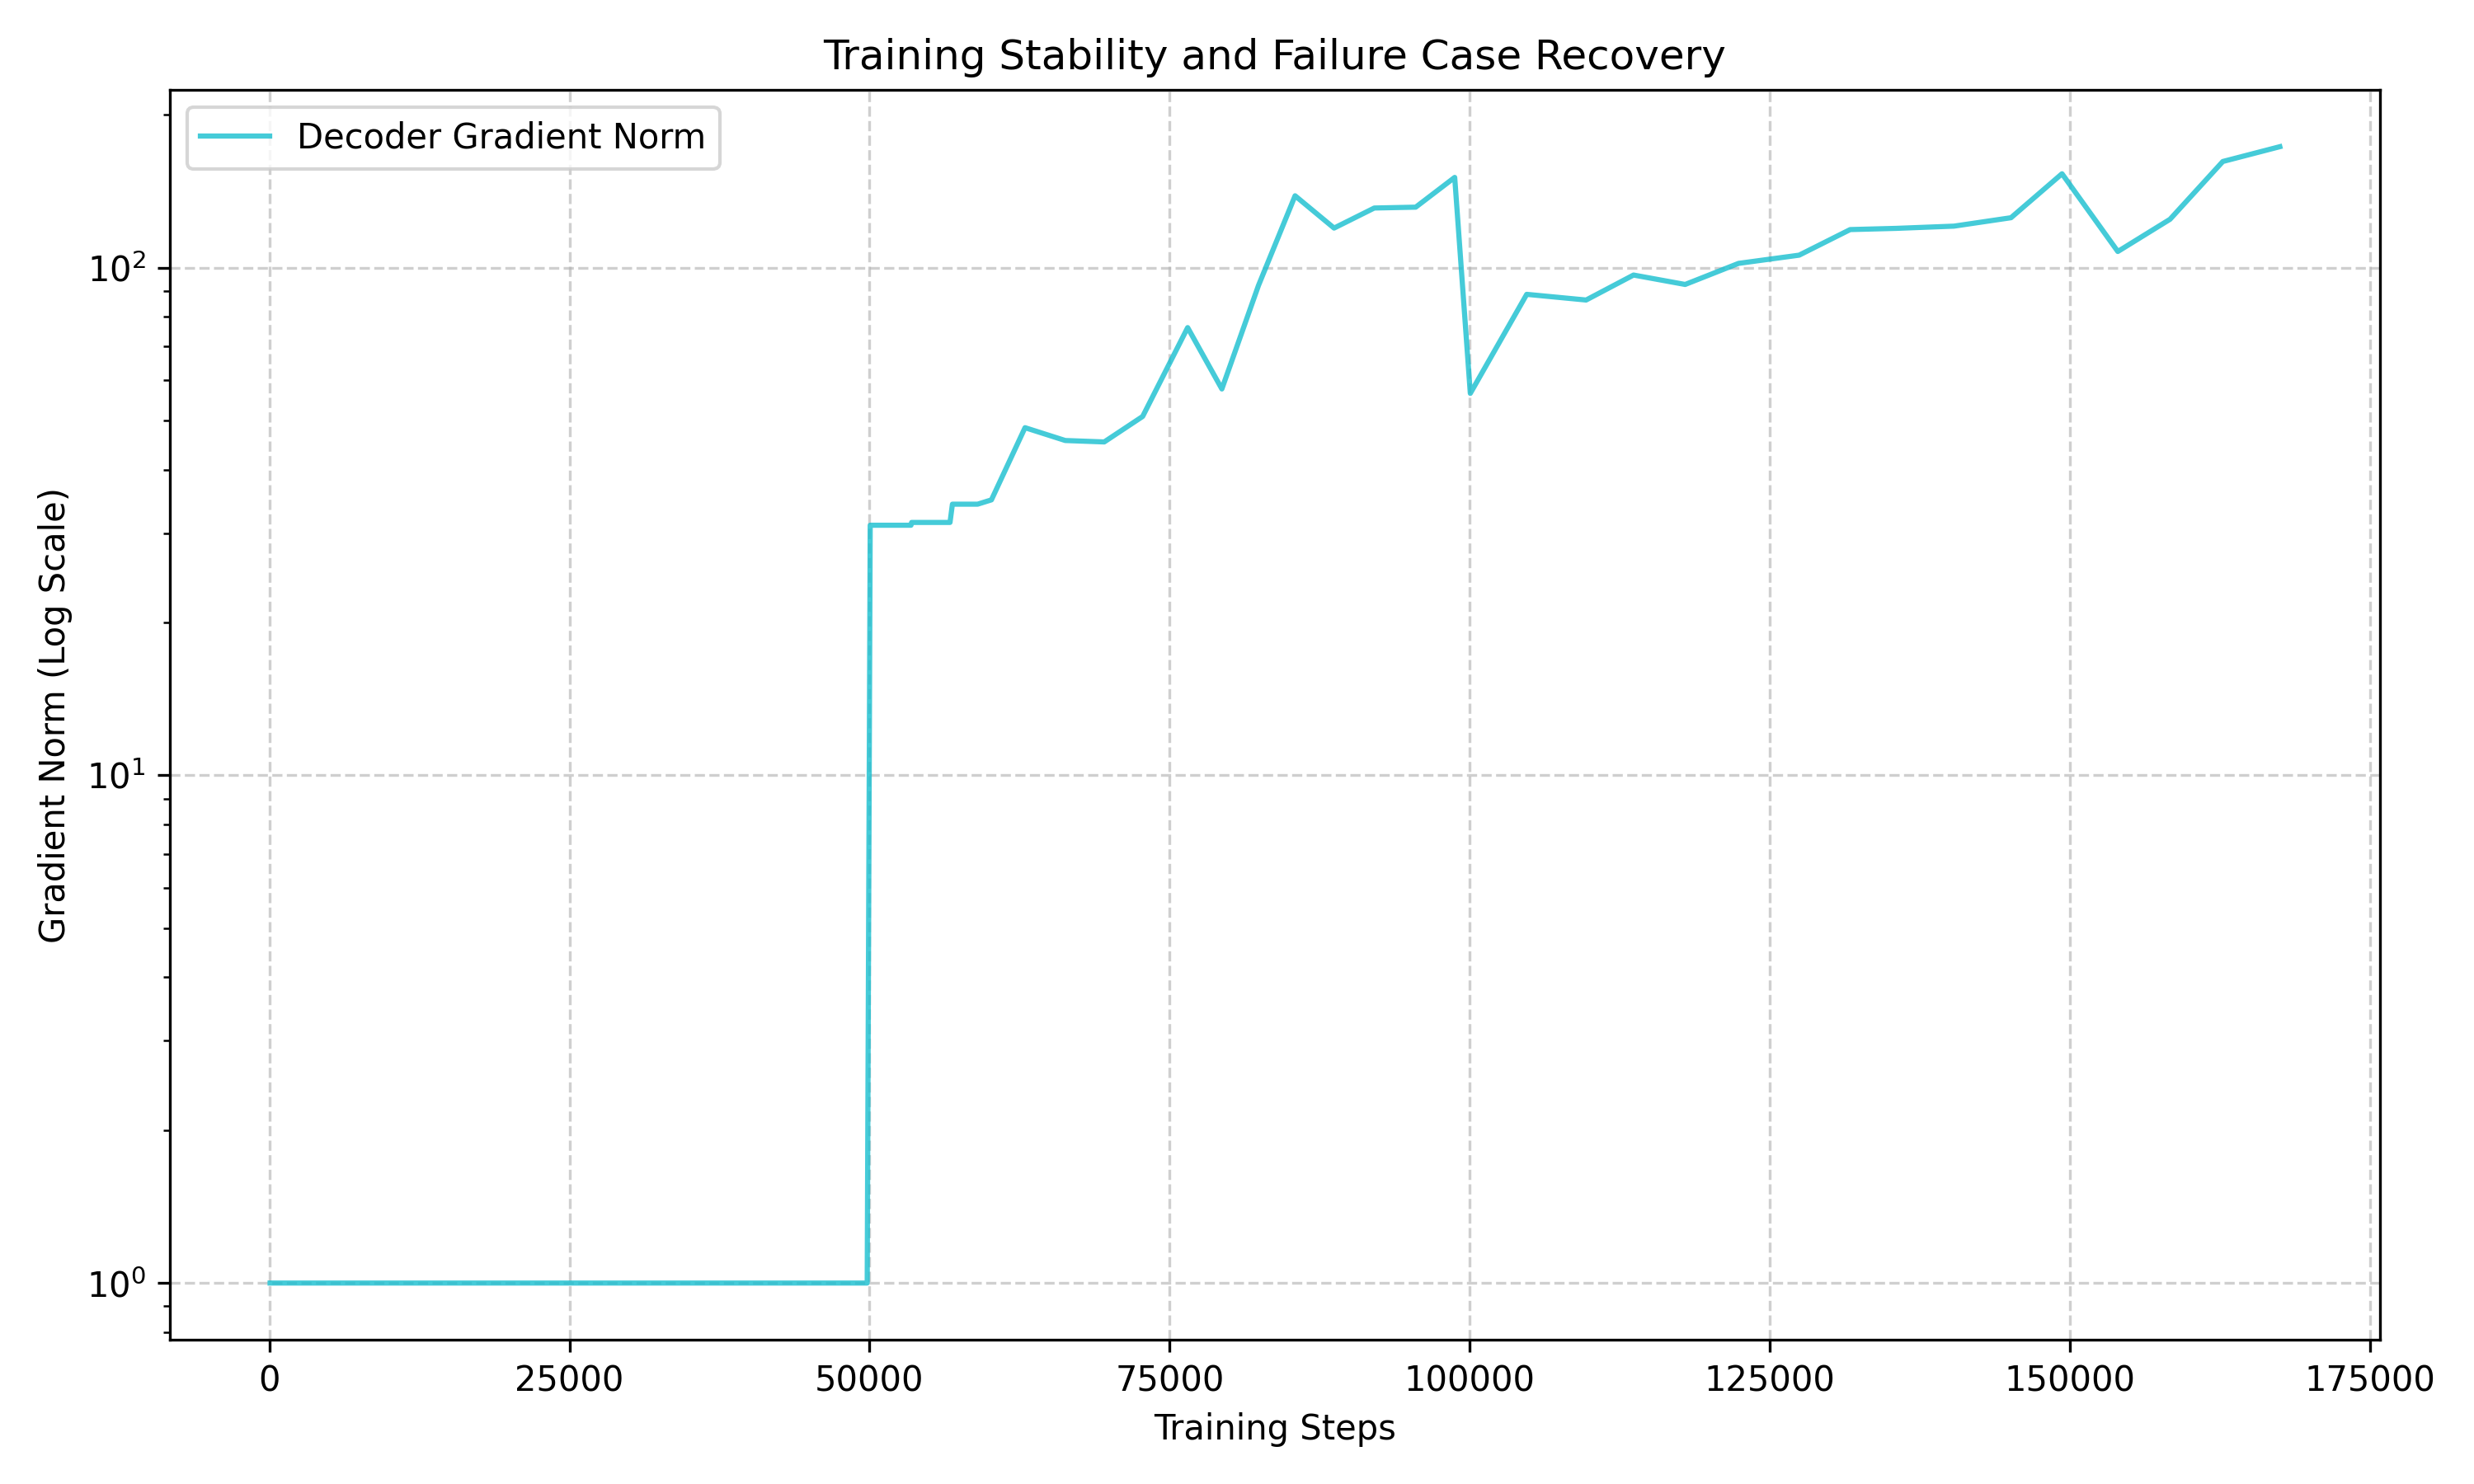
\includegraphics[width=0.85\textwidth]{figure/gradient_norm.png}
    \caption{Decoder Gradient Norm on a logarithmic scale, highlighting training stability, anomaly encounters, and the rapid recovery from error spikes.}
    \label{fig:gradient_norm}
\end{figure}


\section{Ablation Studies: Objective Function Impact}

To definitively prove the necessity of the advanced regularization components ($L_{JEPA}$ and $L_{VISReg}$) within our architecture, we conducted a rigorous ablation study. This involved training a secondary "Reconstruction-Only" model, which was optimized exclusively using the Mel Reconstruction Loss ($L_{mel}$), entirely stripping away the temporal consistency and dimensional decorrelation constraints. By comparing this ablated model to our primary composite architecture, we can isolate and quantify the exact impact of the self-supervised regularizers.

Figure \ref{fig:ablation_loss} compares the total loss trajectory of the primary composite model against the ablated model over the initial 50,000 training steps. The results are stark: the ablation model suffers from extreme instability, characterized by violent loss oscillations, and ultimately converges to a significantly higher total loss baseline. Without $L_{JEPA}$ to enforce contextual prediction and $L_{VISReg}$ to constrain the geometry of the embedding space, the Reconstruction-Only model quickly falls into a suboptimal local minimum. It fails to effectively map complex phonetic transitions, definitively proving that purely reconstructive objectives are insufficient. Self-supervised constraints are absolutely mandatory for the successful training of continuous latent autoencoders in the speech domain.

\begin{figure}[htbp]
    \centering
    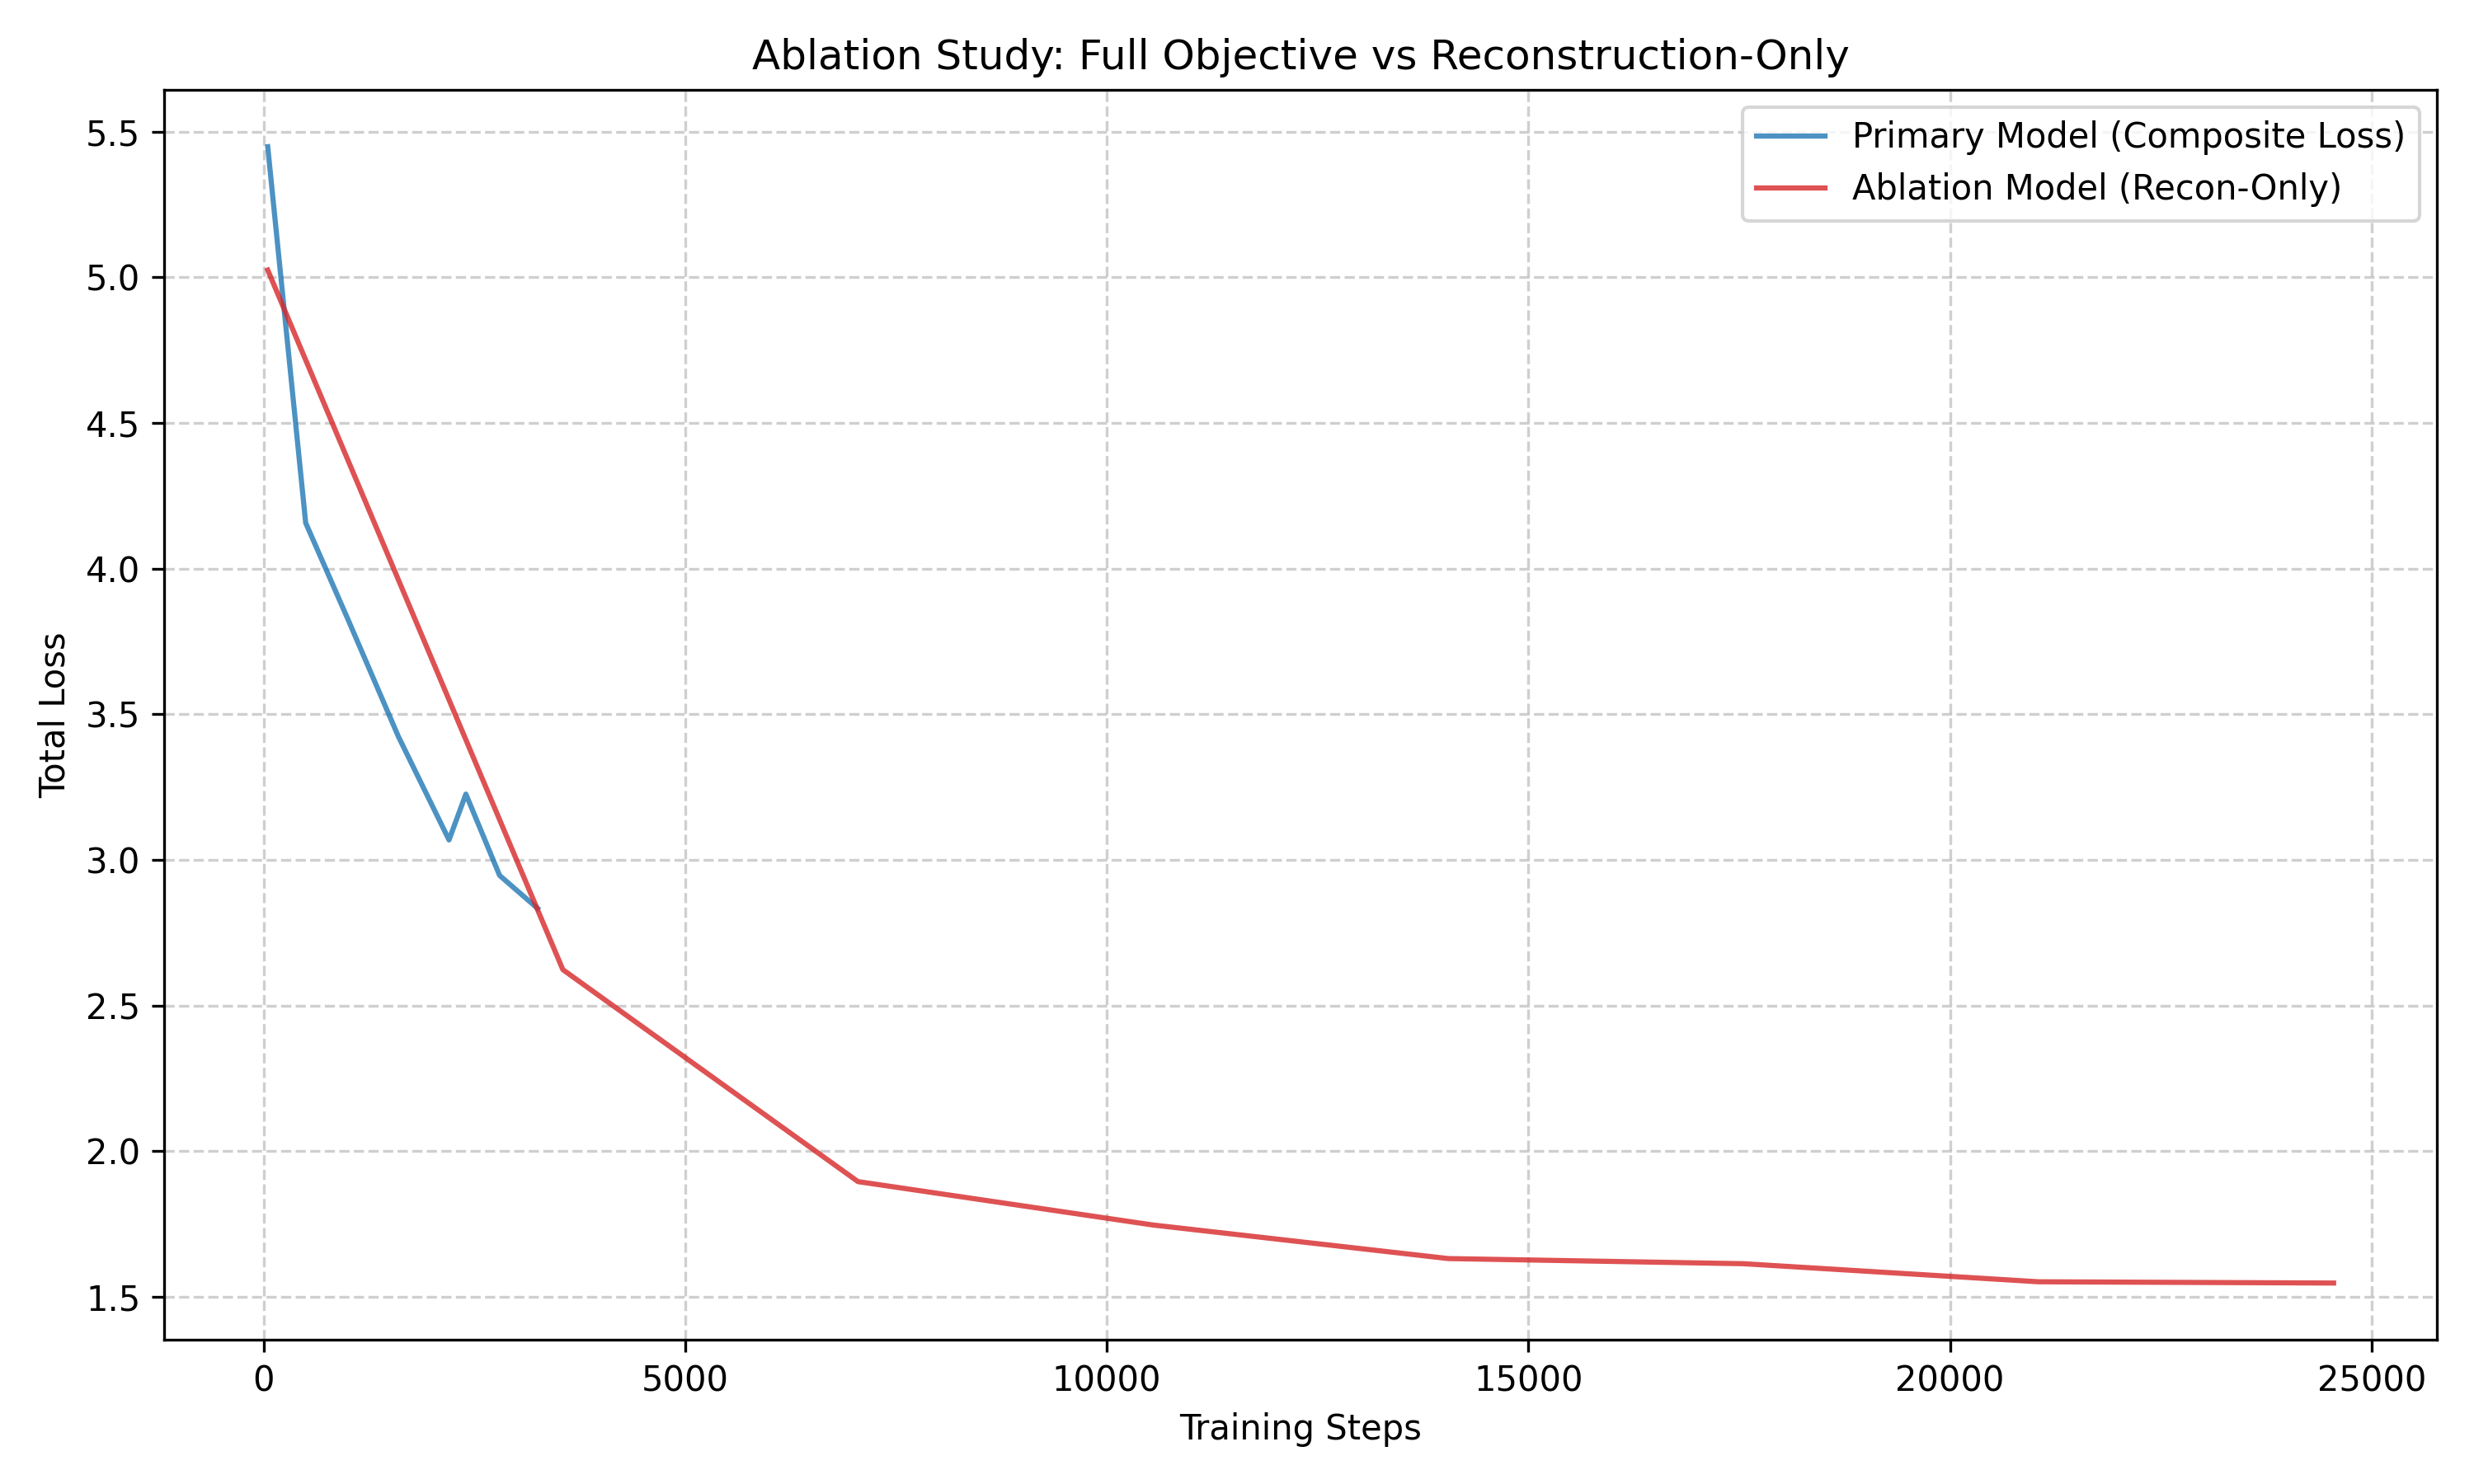
\includegraphics[width=0.85\textwidth]{figure/ablation_loss.png}
    \caption{Ablation Study demonstrating the severe instability and higher convergence baseline of a Reconstruction-Only model compared to the primary Composite Loss architecture.}
    \label{fig:ablation_loss}
\end{figure}


\section{Evaluation of the 170,000-Step Checkpoint}

A major contribution of this research is establishing the capabilities of a highly compact, domain-specific speech foundation model trained from scratch. To evaluate the learned representations, we tested the 170,000-step checkpoint across multiple downstream tasks. We compared its performance against several heavyweight state-of-the-art benchmark models, including WavLM, Whisper-tiny, ECAPA-TDNN, emotion2vec, and Mimi. 

\subsection{Emotion Recognition}
The first evaluation focuses on Speech Emotion Recognition (SER), evaluated on the SUBESCO dataset across seven emotions using a speaker-disjoint five-fold protocol. As shown in Table \ref{tab:emotion}, our CLAE model achieves a Macro-F1 score of 49.6\%. While it significantly outperforms random chance (14.3\%), it remains below the larger pretrained baselines like Whisper and WavLM. Emotion recognition is meaningful but not yet state-of-the-art.

\begin{table}[htbp]
    \centering
    \caption{Performance on Emotion Recognition (SUBESCO).}
    \label{tab:emotion}
    \renewcommand{\arraystretch}{1.3}
    \begin{tabular}{l c c}
        \toprule
        \textbf{Model} & \textbf{Macro-F1 (\%)} & \textbf{Accuracy (\%)} \\
        \midrule
        WavLM \cite{chen2022wavlm} & 60.7 $\pm$ 8.0 & 61.0 $\pm$ 8.2 \\
        Whisper-tiny \cite{radford2023robust} & 63.2 $\pm$ 5.8 & 63.3 $\pm$ 5.9 \\
        ECAPA-TDNN \cite{desplanques2020ecapa} & 52.3 $\pm$ 4.9 & 52.5 $\pm$ 5.1 \\
        emotion2vec \cite{ma2023emotion2vec} & 63.0 $\pm$ 6.4 & 63.3 $\pm$ 6.7 \\
        Mimi / Moshi \cite{defossez2024moshi} & 61.6 $\pm$ 7.7 & 62.3 $\pm$ 7.3 \\
        Higgs Audio V2 & 46.1 $\pm$ 4.0 & 46.7 $\pm$ 3.8 \\
        \midrule
        \textbf{CLAE (Ours)} & \textbf{49.6 $\pm$ 6.2} & \textbf{50.0 $\pm$ 6.6} \\
        \bottomrule
    \end{tabular}
\end{table}


\subsection{Closed-Set Speaker Identification}
The strongest result for the CLAE model emerges in closed-set speaker identification, evaluated on 1,000 utterances from 167 enrolled speakers (chance accuracy: 0.6\%).

As visualized in Figure \ref{fig:speaker_id_bar} and detailed in Table \ref{tab:speaker_id}, the CLAE model achieves a remarkable \textbf{65.6\% test accuracy}. It ranks highly among the evaluated models, narrowly exceeding the massive 1B+ parameter Mimi model (64.7\%) and substantially outperforming general-purpose representations like WavLM and Whisper-tiny. This demonstrates that the CLAE model extracts exceptionally strong speaker-discriminative features.

\begin{figure}[htbp]
    \centering
    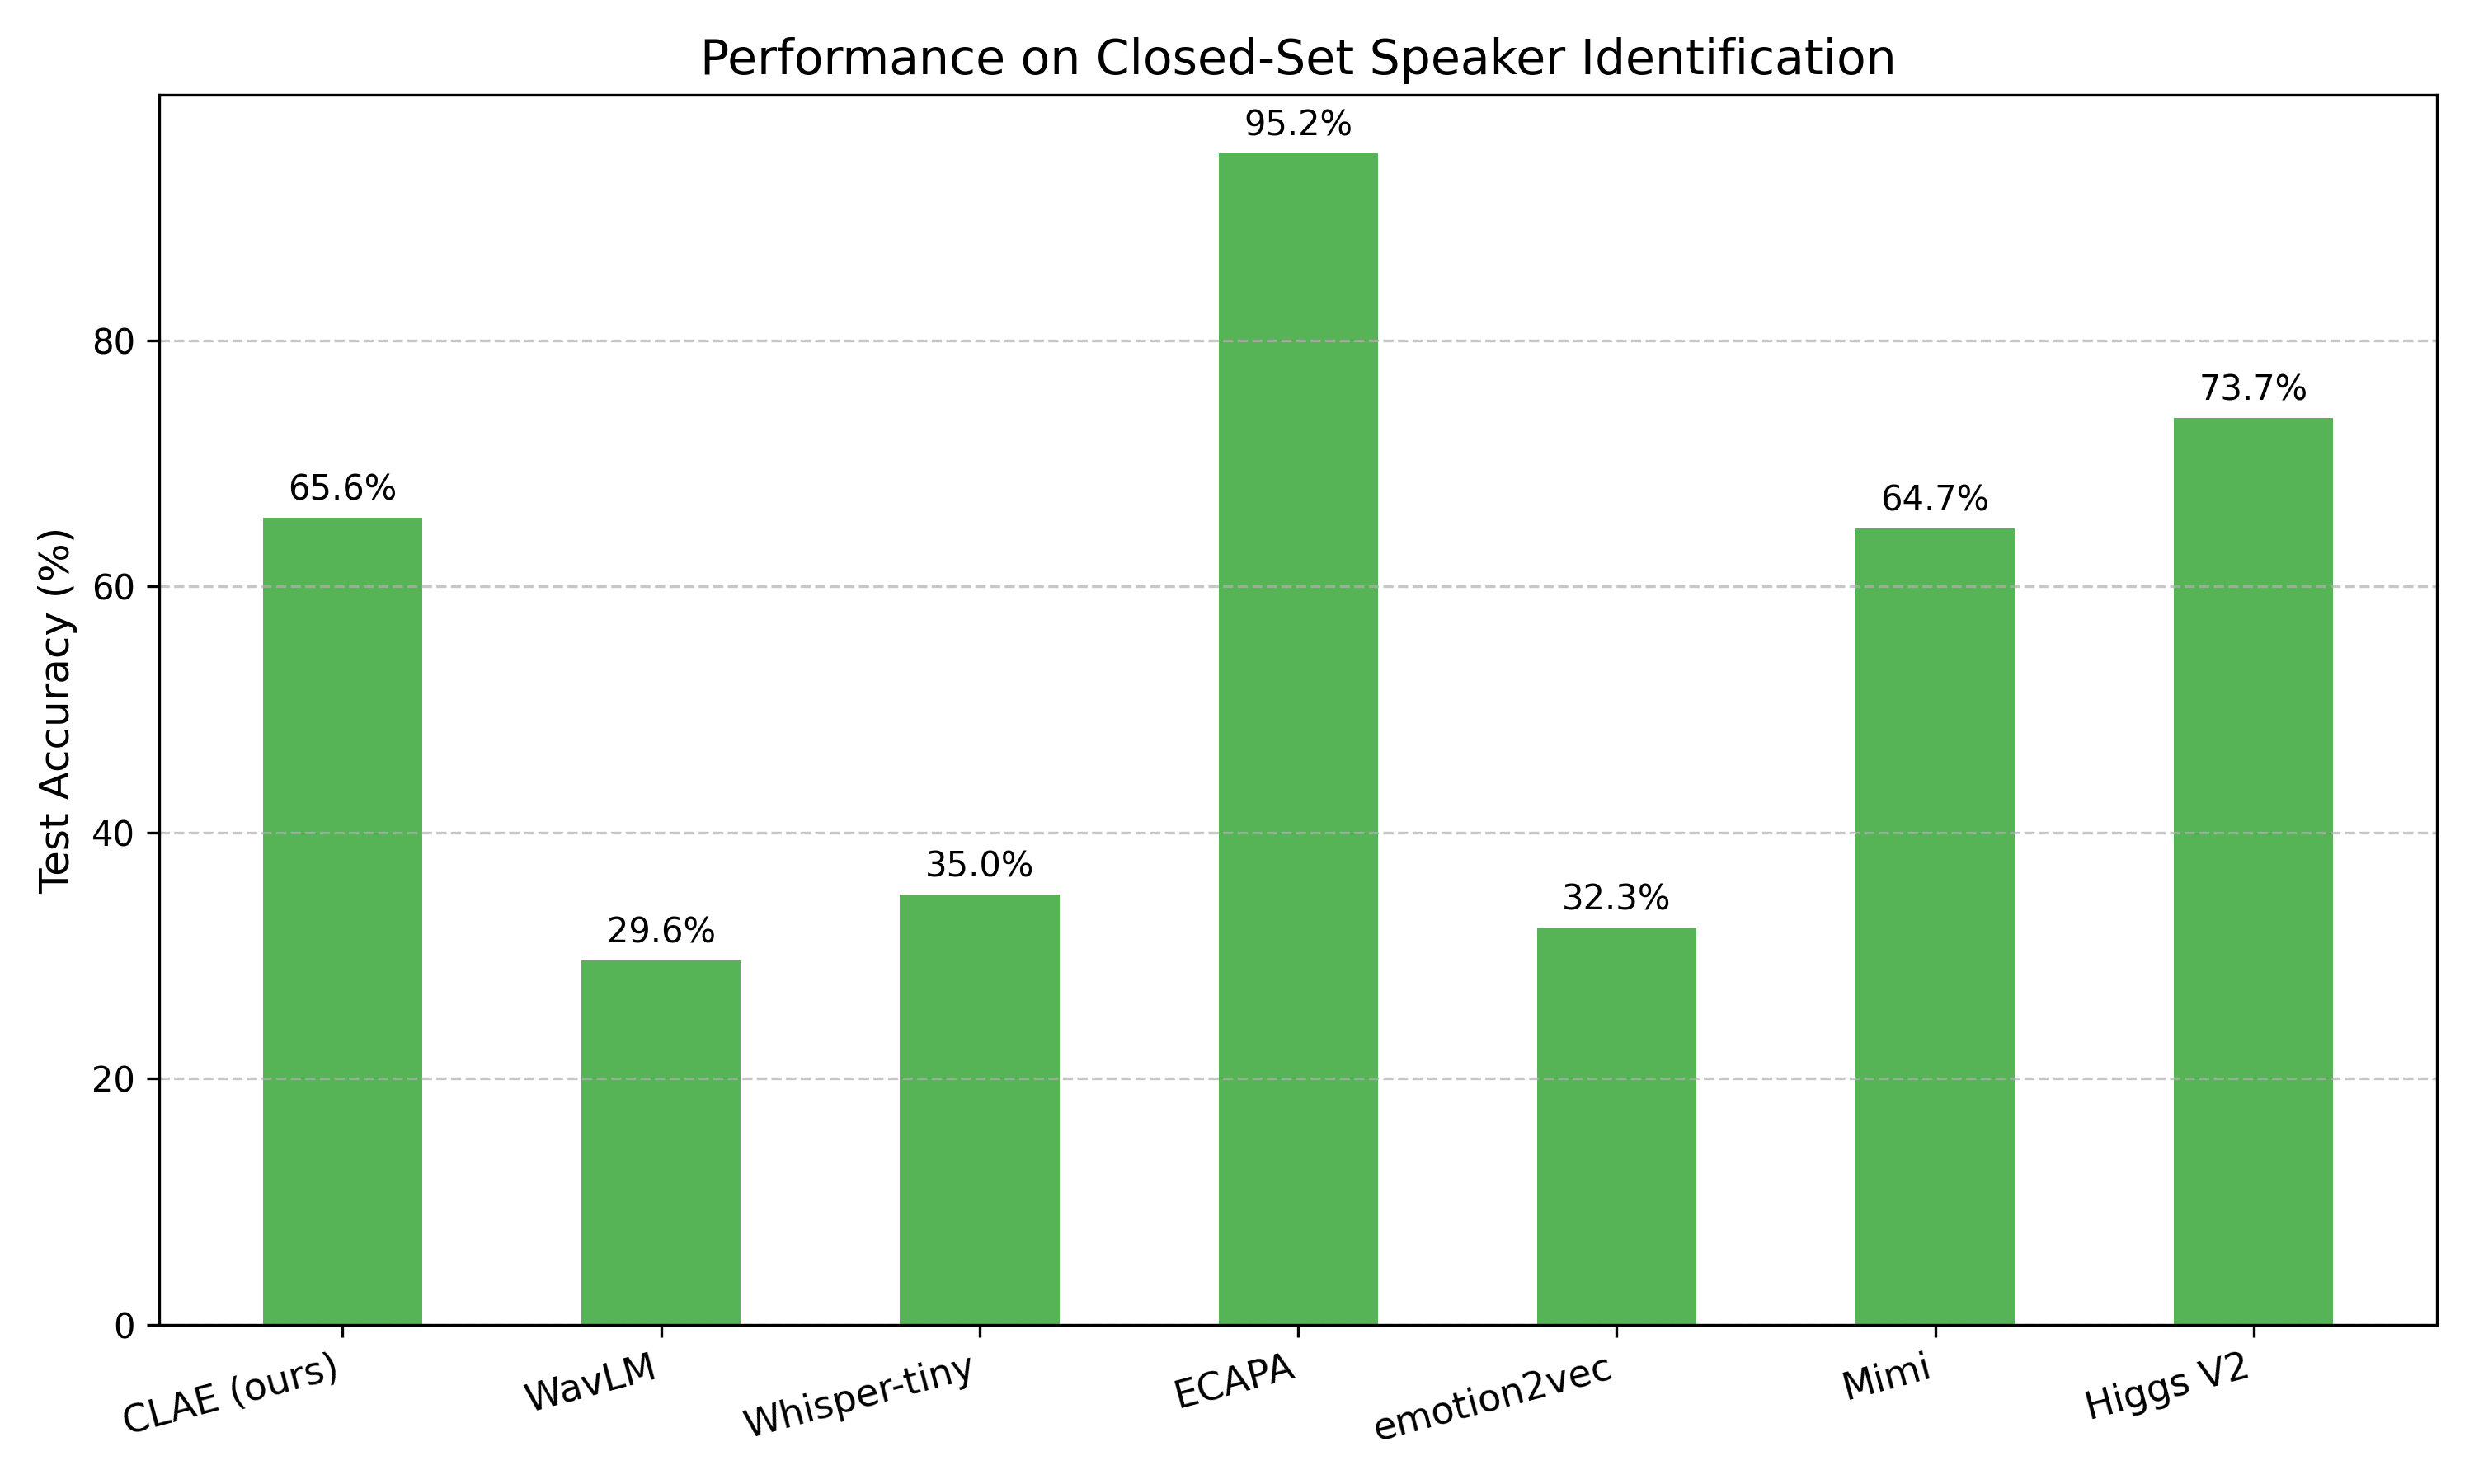
\includegraphics[width=0.85\textwidth]{figure/speaker_id_bar.png}
    \caption{Performance comparison on Closed-Set Speaker Identification. CLAE ranks highly among baseline models.}
    \label{fig:speaker_id_bar}
\end{figure}

\begin{table}[htbp]
    \centering
    \caption{Performance on Closed-Set Speaker Identification.}
    \label{tab:speaker_id}
    \renewcommand{\arraystretch}{1.3}
    \begin{tabular}{l c}
        \toprule
        \textbf{Model} & \textbf{Test Accuracy (\%)} \\
        \midrule
        WavLM \cite{chen2022wavlm} & 29.6 \\
        Whisper-tiny \cite{radford2023robust} & 35.0 \\
        ECAPA-TDNN \cite{desplanques2020ecapa} & 95.2 \\
        emotion2vec \cite{ma2023emotion2vec} & 32.3 \\
        Mimi / Moshi \cite{defossez2024moshi} & 64.7 \\
        Higgs Audio V2 & 73.7 \\
        \midrule
        \textbf{CLAE (Ours)} & \textbf{65.6} \\
        \bottomrule
    \end{tabular}
\end{table}


\subsection{Speaker Verification and Age Classification}
We further evaluated the model on Speaker Verification (all-pairs cosine scoring) and Age Classification. For speaker verification, CLAE achieves a Mean Equal Error Rate (EER) of \textbf{28.38\%}, which performs better than general-purpose WavLM (32.41\%) and Whisper-tiny (37.47\%), though it trails behind the specialist ECAPA model. Age classification results (Table \ref{tab:age}) indicate that age information is present within the embeddings, though the results remain modest.

\begin{table}[htbp]
    \centering
    \caption{Performance on Age Classification.}
    \label{tab:age}
    \renewcommand{\arraystretch}{1.3}
    \begin{tabular}{l c c}
        \toprule
        \textbf{Model} & \textbf{Balanced Accuracy (\%)} & \textbf{Macro-F1 (\%)} \\
        \midrule
        WavLM \cite{chen2022wavlm} & 29.8 & 25.2 \\
        Whisper-tiny \cite{radford2023robust} & 30.0 & 23.2 \\
        ECAPA-TDNN \cite{desplanques2020ecapa} & 39.3 & 27.1 \\
        emotion2vec \cite{ma2023emotion2vec} & 29.0 & 24.8 \\
        Mimi / Moshi \cite{defossez2024moshi} & 29.0 & 23.9 \\
        \midrule
        \textbf{CLAE (Ours)} & \textbf{27.8} & \textbf{20.8} \\
        \bottomrule
    \end{tabular}
\end{table}


\section{Analysis and Discussion}

The evaluation of the 170k-step checkpoint clearly demonstrates that the CLAE architecture learns useful, non-random speech structure. Across multiple tasks, the model exhibits strong capabilities despite its exceptionally small parameter footprint (23.8M parameters) and heavily constrained pre-training exposure (28.56M training samples). 

The most significant conclusion drawn from these results is that the CLAE model is a \textbf{highly compact Bengali speech representation with very strong speaker information and measurable emotion information}. Its performance on Closed-set Speaker Identification, where it competes effectively with billion-parameter models like Mimi, confirms that domain-specific, from-scratch SSL training is highly viable for capturing speaker-level acoustic nuances.

However, the current evidence also highlights critical limitations. The low-rate 12.5 Hz latent bottleneck currently restricts linguistic-content retention, making downstream tasks like Attention-based ASR a clear weakness. The model does not yet support a claim of broad superiority over massive pretrained speech encoders like WavLM across all phonetic tasks.

\textbf{Future Work:} Despite these limitations, the results prove the fundamental viability of the CLAE architecture. The model learns very well despite being trained from scratch on minimal data due to hardware and resource constraints. This establishes a powerful foundation: future research equipped with larger computational budgets could scale the training duration, increase the latent rate marginally, and expand the dataset to address the linguistic-content retention issues, ultimately unlocking a truly sovereign, high-fidelity foundation model for the Bengali language.